%
\section{Testen}
\definecolor{bluekeywords}{rgb}{0.13,0.13,1}
\definecolor{greencomments}{rgb}{0,0.5,0}
\definecolor{redstrings}{rgb}{0.9,0,0}
\definecolor{light-gray}{gray}{0.96}
\lstset{language=[Sharp]C,
	showspaces=false,
	showtabs=false,
	breaklines=true,
	showstringspaces=false,
	breakatwhitespace=true,
	escapeinside={(*@}{@*)},
	commentstyle=\color{greencomments},
	keywordstyle=\color{bluekeywords},
	stringstyle=\color{redstrings},
	basicstyle=\ttfamily,
	tabsize=2,
	backgroundcolor=\color{light-gray}
}
In diesem Kapitel wollen wir die Software C\# Essentials durch effiziente Test auf Fehler prüfen. Bei der Betrachtung des Codes ist uns aufgefallen, das der Entwickler Dustin Campbell Qualitativ hochwertigen Code geschrieben hat und auch eine sehr gute Testabdeckung besteht. Im folgenden möchten wir jedoch nicht nur jede einzelne Methode testen, sondern auch gelernte Inhalte aus der Vorlesung, wie Graph Coverage, umsetzen.\\
Vorab steht für uns fest, dass wir keine Input Coverage gezielt betrachten werden, weil die Methoden alle Codeschnipsel oder Teile von diesen bekommen und wir festgestellt haben, dass der Entwickler für jeden Fall ein Test mit einem Codeschnipsel programmiert hat. Somit hat der Entwickler an dieser Stelle schon gute Arbeit geleistet.\\
Zudem haben wir keine Möglichkeit Syntax Coverage umzusetzen, da wir in dem Projekt keine strikte Syntax oder Grammatik haben.

\subsection{Testen der Methode \texttt{IsWithinConstructorOf}}
In C\# 6 können Auto-Properties ohne Setter deklariert werden.\cite{csharp6} C\# Essentials überprüft, ob der Setter weggelassen werden kann und teilt dies gegebenenfalls dem Benutzer mit. Die Methode \texttt{IsWithinConstructorOf} überprüft dabei, ob das Setzen des Auto-Properties im Konstruktor stattfindet. Die statische Analyse ergab, dass diese Methode sehr Komplex und damit sehr fehleranfällig ist. Daher haben wir uns entschlossen diese genauer zu testen. Aus dem in Listing \ref{lst:code-IsWithinConstructorOf} gezeigten Code haben wir, den in Abbildung~\ref{fig:graph-constructor} dargestellten, Kontrollflussgraphen erstellt. Anschließend haben wir die in Listing \ref{lst:coverage-IsWithinConstructorOf} zu sehenden Testpfade für unterschiedliche Coverage Kriterien entwickelt.\\
\begin{figure}[h]
	\centering
	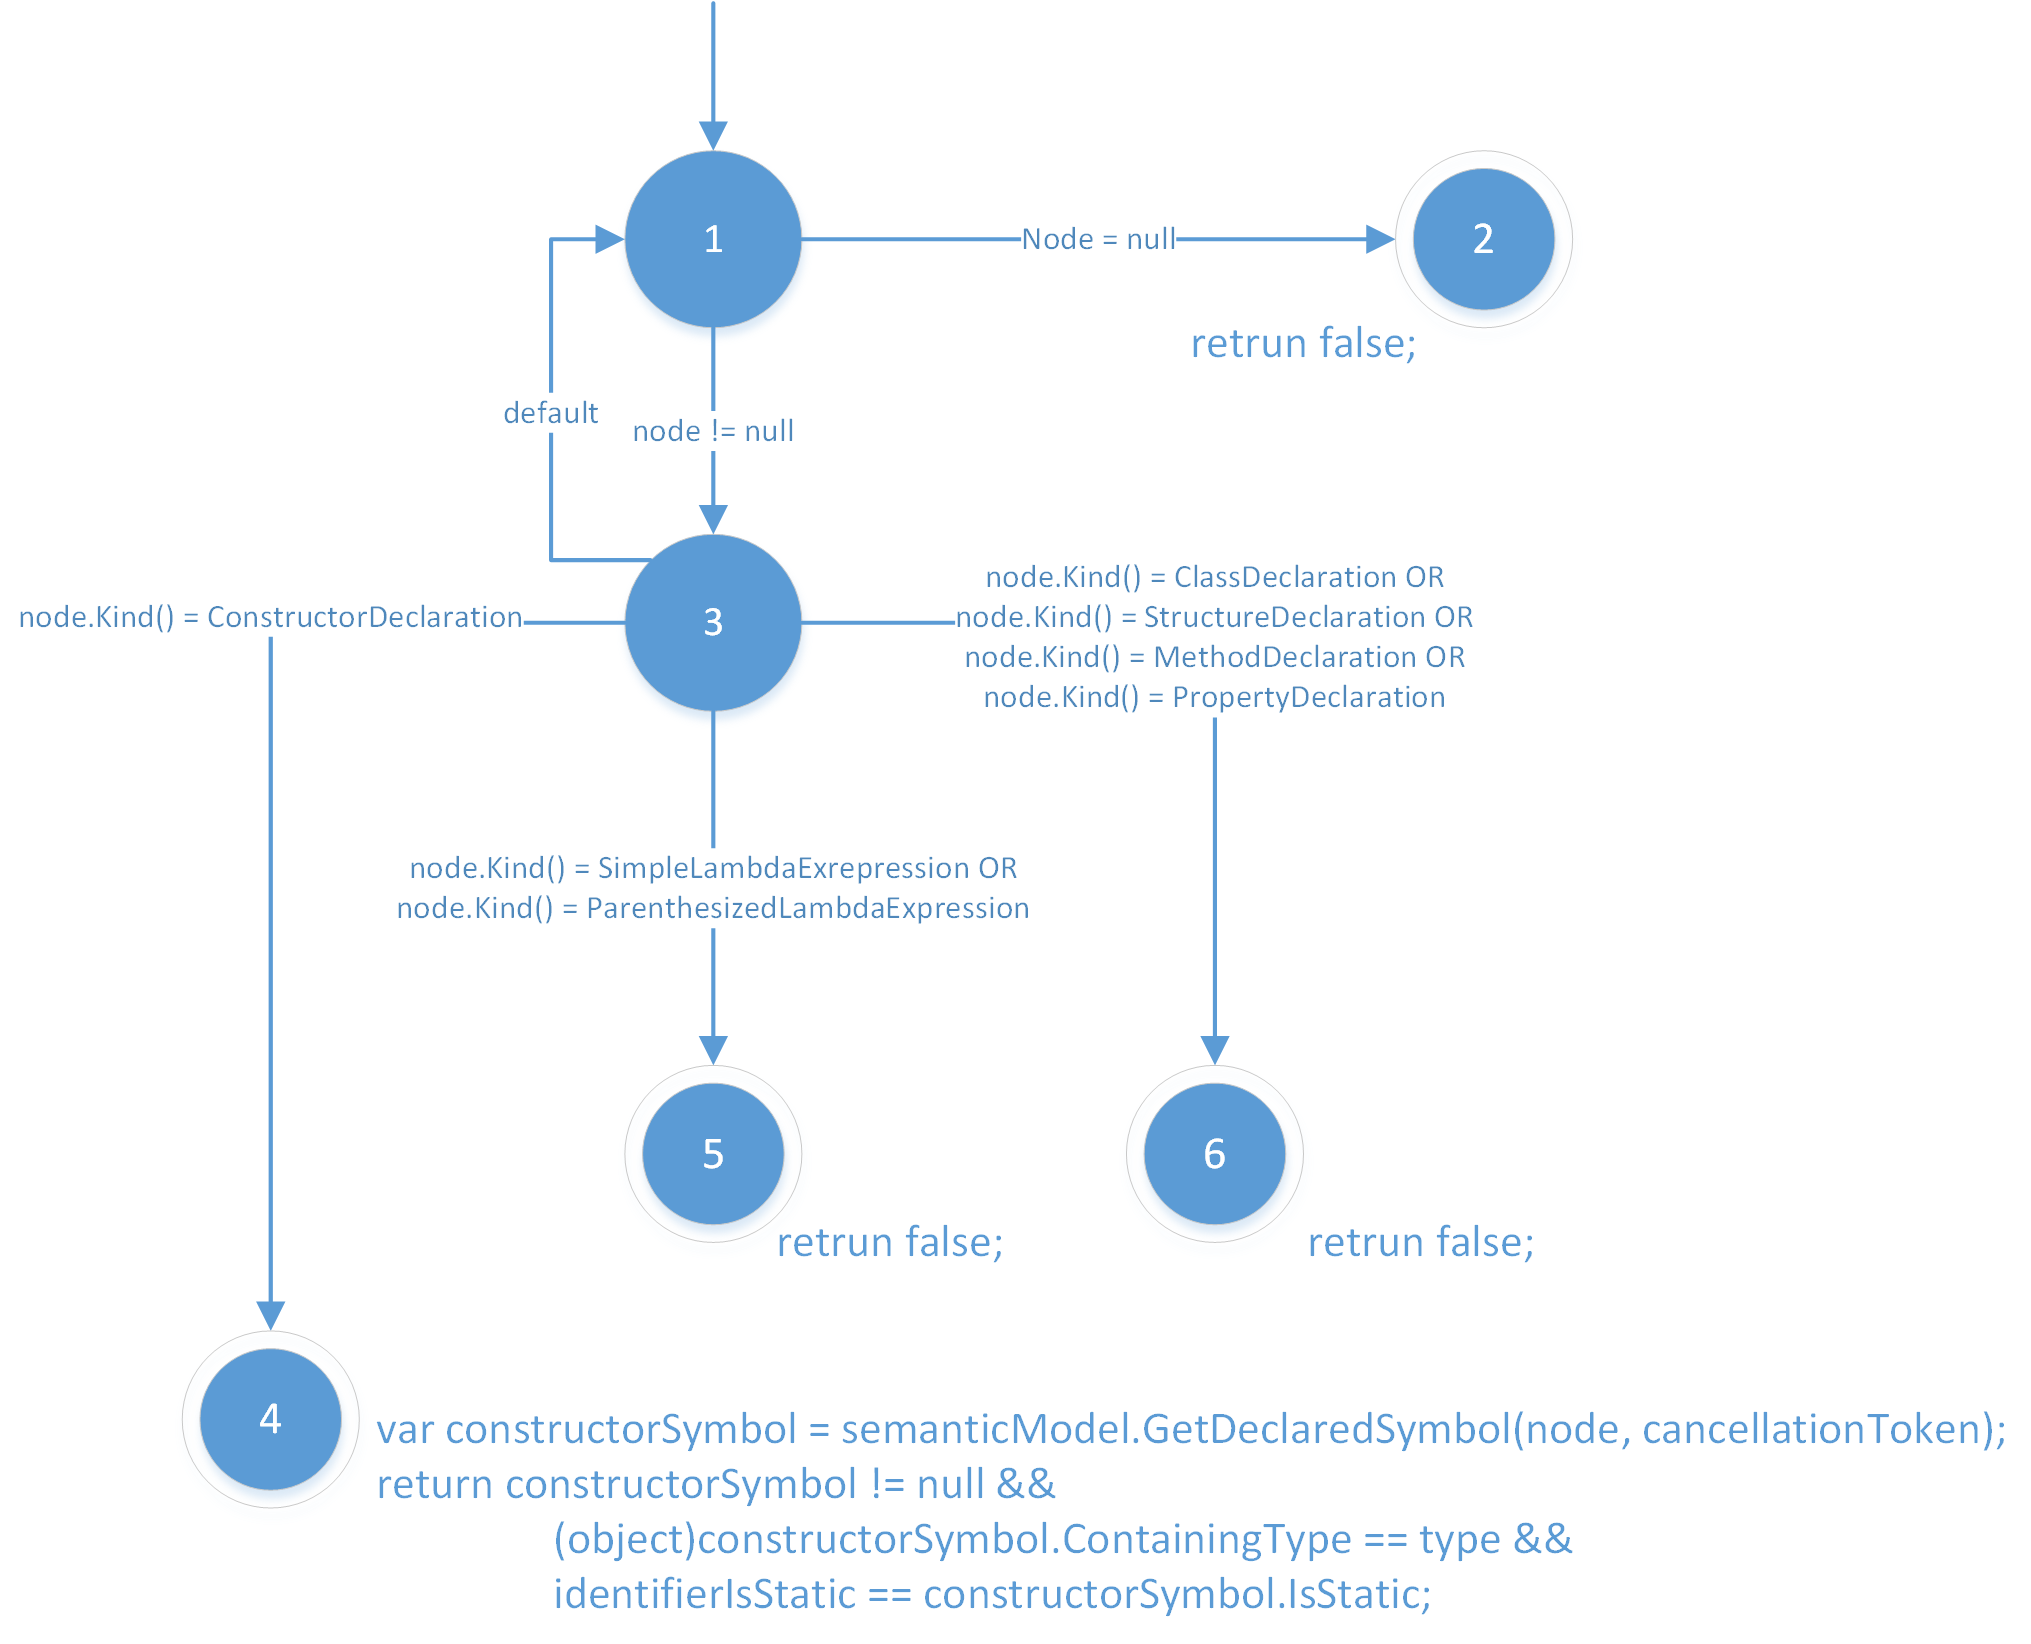
\includegraphics[width=\textwidth]{images/GraphIsWithinConstructorOf.png}
	\caption{Graph für die Methode \texttt{IsWithinConstructorOf}}
	\label{fig:graph-constructor}
\end{figure}
\begin{lstlisting}[caption={Coverage für die Mehtode \texttt{IsWithinConstructorOf}},
label=lst:coverage-IsWithinConstructorOf]
Node Coverage:
TR = {1,2,3,4,5,6}
Example Test Paths = [1,3,4], [1,3,5], [1,3,6]

Edge Coverage:
TR = {(1,2), (1,3), (3,1), (3,4), (3,5), (3,6)}
Example Test Paths = [1,3,1,2], [1,3,4], [1,3,5], [1,3,6]

Edge Pair Coverage:
TR = {[1,3,1], [1,3,4], [1,3,5], [1,3,6], [3,1,3], [3,1,2]}
Example Test Paths = [1,3,1,3,1,2], [1,3,4], [1,3,5], [1,3,6]

Prime Path Coverage:
TR = {[1,3,4], [1,3,5], [1,3,6], [3,1,2], [3,1,3], [1,3,1]}
Example Test Paths: [1,3,1,3,1,2], [1,3,4], [1,3,4], [1,3,5]
\end{lstlisting}
\vspace{1ex}
Zu erkennen ist, dass Edge Pair und Prime Path Coverage die selben Testpfade besitzen. Abschließend haben wir für jeden Testpfad der Prime beziehungsweise Edge Pair Coverage einen Test programmiert. Anhand eines Beispiels sollen die Tests erläutert werden. Die in Listing \ref{lst:code-AutoPropUsedInLambdaInConstructorCannotBeReadonly} gezeigte Testmethode \texttt{AutoPropUsedInLambdaInConstructorCannotBeReadonly} deckt den Pfad \texttt{[1,3,5]} ab. In der Testmethode wird die Methode \texttt{IsWithinConstructorOf} mit dem im Test definierten Codeschnipsel geprüft. Beim Schleifendurchlauf trifft der Fall \texttt{ParenthesizedLambdaExpression} zu. Die Methode gibt \texttt{false} zurück. Deshalb hat C\# Essentials in diesem Fall keine Verbesserungsvorschläge für den Nutzer und der Test ist erfüllt.
\begin{lstlisting}[caption={Mehtode \texttt{IsWithinConstructorOf}},
label=lst:code-IsWithinConstructorOf]
private static bool IsWithinConstructorOf(SyntaxNode node, INamedTypeSymbol type, bool identifierIsStatic, SemanticModel semanticModel, CancellationToken cancellationToken)
{
// Are we in a constructor?
for (; node != null; node = node.Parent)
{
switch (node.Kind())
{
case SyntaxKind.ConstructorDeclaration:
// In a constructor. Is it the constructor for the type that contains the property?
var constructorSymbol = semanticModel.GetDeclaredSymbol(node, cancellationToken);
return constructorSymbol != null && (object)constructorSymbol.ContainingType == type && identifierIsStatic == constructorSymbol.IsStatic;
// If it's in a lambda expression, even if in a constructor, then it counts as a non-constructor case.
case SyntaxKind.SimpleLambdaExpression:
case SyntaxKind.ParenthesizedLambdaExpression:
return false;
// Early out cases. There are many others, but these are the common ones.
case SyntaxKind.ClassDeclaration:
case SyntaxKind.StructDeclaration:
case SyntaxKind.MethodDeclaration:
case SyntaxKind.PropertyDeclaration:
return false;
}
}
return false;
}
\end{lstlisting}
\begin{lstlisting}[caption={Mehtode \texttt{AutoPropUsedInLambdaInConstructorCannotBeReadonly}},
label=lst:code-AutoPropUsedInLambdaInConstructorCannotBeReadonly]
[Test]
public void AutoPropUsedInLambdaInConstructorCannotBeReadonly()
{
const string code = @"
class C
{
public int P { get; private set; }

public C()
{
var f = new Action(() => P = 2);
}
}";
NoDiagnostic(code, DiagnosticIds.UseGetterOnlyAutoProperty);
}
\end{lstlisting}
\subsection{Testen der Methode \texttt{UpdatingExpression}}
Die statische ergab auch bei der Methode \texttt{UpdatingExpression} eine hohe Komplexität. Daher wollen wir auch auf diese genauer eingehen. Die Methode sucht genau wie \texttt{IsWithinConstructorOf}, ob ein Setter einer Auto-Property existiert. Allerdings sucht sie außerhalb des Konstruktors. Anhand des Codes er Methode aus Listing \ref{lst:code-UpdatingExpression} haben wir den Kontrollflussgraphen in Abbildung \ref{fig:graph-UpdatingExpression} erstellt und dann die Coverage Kriterien in Listing \ref{lst:coverage-UpdatingExpression} aufgestellt.
\begin{lstlisting}[caption={Coverage für die Mehtode \texttt{UpdatingExpression}},
label=lst:coverage-UpdatingExpression]
Node Coverage:
TR = {1,2,3,4,5,6,7,8,9}
Example Test Paths = [1,2,3,4], [1,2,3,5], [1,2,3,6], [1,2,3,7], [1,2,8]

Edge Coverage:
TR = {(1,2), (2,3), (2,8), (3,2), (3,4), (3,5), (3,6), (3,7)}
Example Test Paths = [1,2,3,4], [1,2,3,5], [1,2,3,6], [1,2,3,7], [1,2,3,2,8]

Edge Pair Coverage:
TR = {[1,2,3], [1,2,8], [2,3,2], [2,3,4], [2,3,5], [2,3,6], [2,3,7], [3,2,3], [3,2,8]}
Example Test Paths = [1,2,3,2,3,4], [1,2,3,5], [1,2,3,6], [1,2,3,7], [1,2,8]

Prime Path Coverage:
TR = {[1,2,3,4], [1,2,3,5], [1,2,3,6], [1,2,3,7], [1,2,8], [3,2,8], [3,2,3], [2,3,2]}
Example Test Paths: [1,2,3,2,3,2,8], [1,2,3,4], [1,2,3,5], [1,2,3,6], [1,2,3,7], [1,2,8]
\end{lstlisting}
\begin{figure}[h]
	\centering
	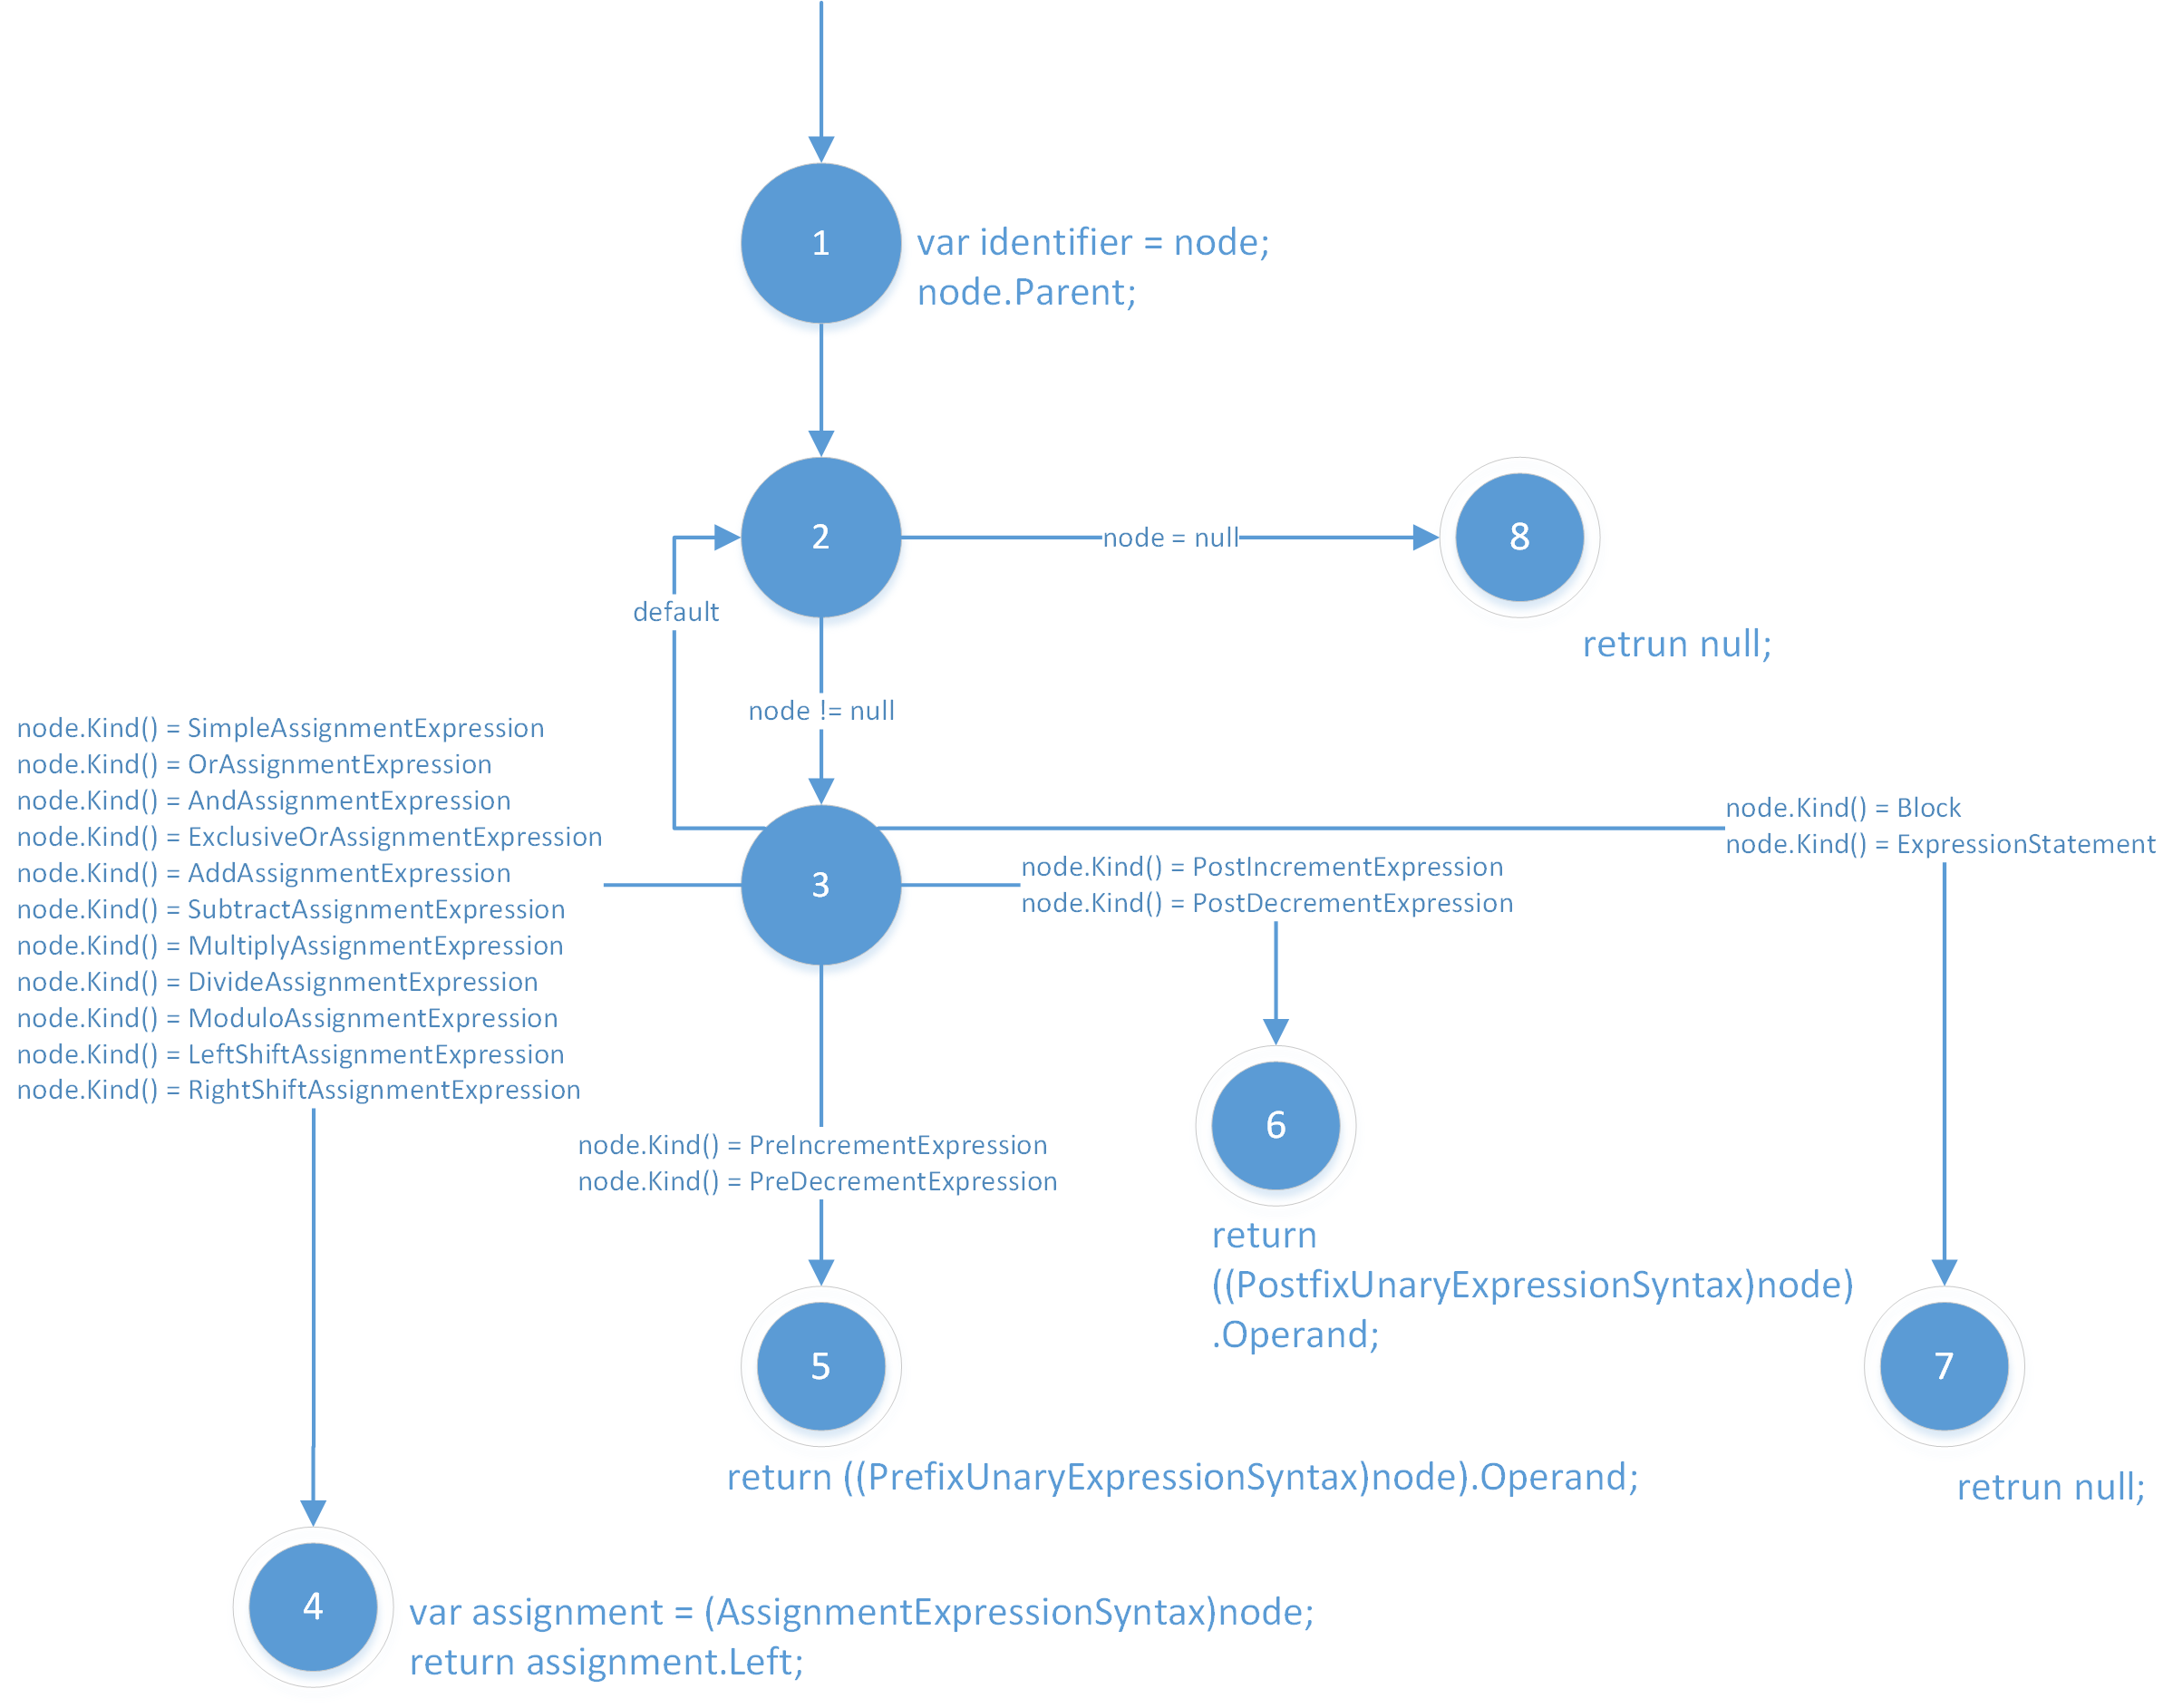
\includegraphics[width=\textwidth]{images/GraphUpdatingExpression.png}
	\caption{Graph für die Methode \texttt{UpdatingExpression}}
	\label{fig:graph-UpdatingExpression}
\end{figure}
Als nächstes haben wir für jeden Testpfad der Prime Coverage einen Test programmiert. Auf Grund der Ähnlichkeit der Methoden \texttt{UpdatingExpression} und \texttt{IsWithinConstructorOf} und ihrer Testmethoden verzichten wir an dieser Stelle auf eine genaue beispielhafte Erläuterung eines Tests.\newpage
\begin{lstlisting}[caption={Mehtode \texttt{UpdatingExpression}},
label=lst:code-UpdatingExpression]
private static SyntaxNode UpdatingExpression(SyntaxNode node)
{
	var identifier = node;
 	for (node = node.Parent; node != null; node = node.Parent)
 	{
 		switch (node.Kind())
 		{
 			// Simple or compound assignment
 			case SyntaxKind.SimpleAssignmentExpression:
 			case SyntaxKind.OrAssignmentExpression:
 			case SyntaxKind.AndAssignmentExpression:
 			case SyntaxKind.ExclusiveOrAssignmentExpression:
 			case SyntaxKind.AddAssignmentExpression:
 			case SyntaxKind.SubtractAssignmentExpression:
 			case SyntaxKind.MultiplyAssignmentExpression:
 			case SyntaxKind.DivideAssignmentExpression:
 			case SyntaxKind.ModuloAssignmentExpression:
 			case SyntaxKind.LeftShiftAssignmentExpression:
 			case SyntaxKind.RightShiftAssignmentExpression:
 			var assignment = (AssignmentExpressionSyntax)node;
 			return assignment.Left;
 			
 			// Prefix unary expression
 			case SyntaxKind.PreIncrementExpression:
 			case SyntaxKind.PreDecrementExpression:
 			return ((PrefixUnaryExpressionSyntax)node).Operand;
 			
 			// Postfix unary expression
 			case SyntaxKind.PostIncrementExpression:
 			case SyntaxKind.PostDecrementExpression:
 			return ((PostfixUnaryExpressionSyntax)node).Operand;
 			
 			// Early loop termination
 			case SyntaxKind.Block:
 			case SyntaxKind.ExpressionStatement:
 			return null;
 		}
 	}
 	
	return null;
}
\end{lstlisting}
\subsection{Testen der Methode \texttt{IsValidStringFormatMethod}}
C\# 6 unterstützt interpolated Strings. Anstatt in der \texttt{String.Format} Methode Platzhalter zu verwenden, um Variablen einzufügen, können diese nun direkt im String verwendet werden.\cite{csharp6} C\# Essentials gibt dem Benutzer Vorschläge, wie er die neuen interpolated Strings verwendet. Die Methode \texttt{String.Format} überprüft in diesem Zusammenhang, wann es sich um ein valide \texttt{String.Format} Methode handelt.\\
Auch beim Testen dieser Methode haben wir zu erst den Kontrollflussgraphen, wie in Abbildung \ref{fig:graph-validstring} zu sehen, aus dem in Listing \ref{lst:code-IsValidStringFormatMethod} abgebildeten Code erzeugt. Anschließend haben wir die in Listing \ref{lst:coverage-IsValidStringFormatMethod} dargestellten Coverage Kriterien aufgestellt.

\begin{lstlisting}[caption={Coverage für die Mehtode \texttt{IsValidStringFormatMethod}},
label=lst:coverage-IsValidStringFormatMethod]
Node Coverage:
TR = {1,2,3,4,5,6,7}
Example Test Paths = [1,2], [1,3,4], [1,3,5,6], [1,3,5,7]

Edge Coverage:
TR = {(1,2), (1,3), (3,4), (3,5), (5,6), (5,7)}
Example Test Paths = [1,2], [1,3,4], [1,3,5,6], [1,3,5,7]
Edge Pair Coverage:
TR = {[1,2], [1,3,4], [1,3,5], [3,5,6], [3,5,7]}
Example Test Paths = [1,2], [1,3,4], [1,3,5,6], [1,3,5,7]

Prime Path Coverage:
TR = {[1,2], [1,3,4], [1,3,5,6], [1,3,5,7]}
Example Test Paths: [1,2], [1,3,4], [1,3,5,6], [1,3,5,7]
\end{lstlisting}
\begin{figure}[h]
	\centering
	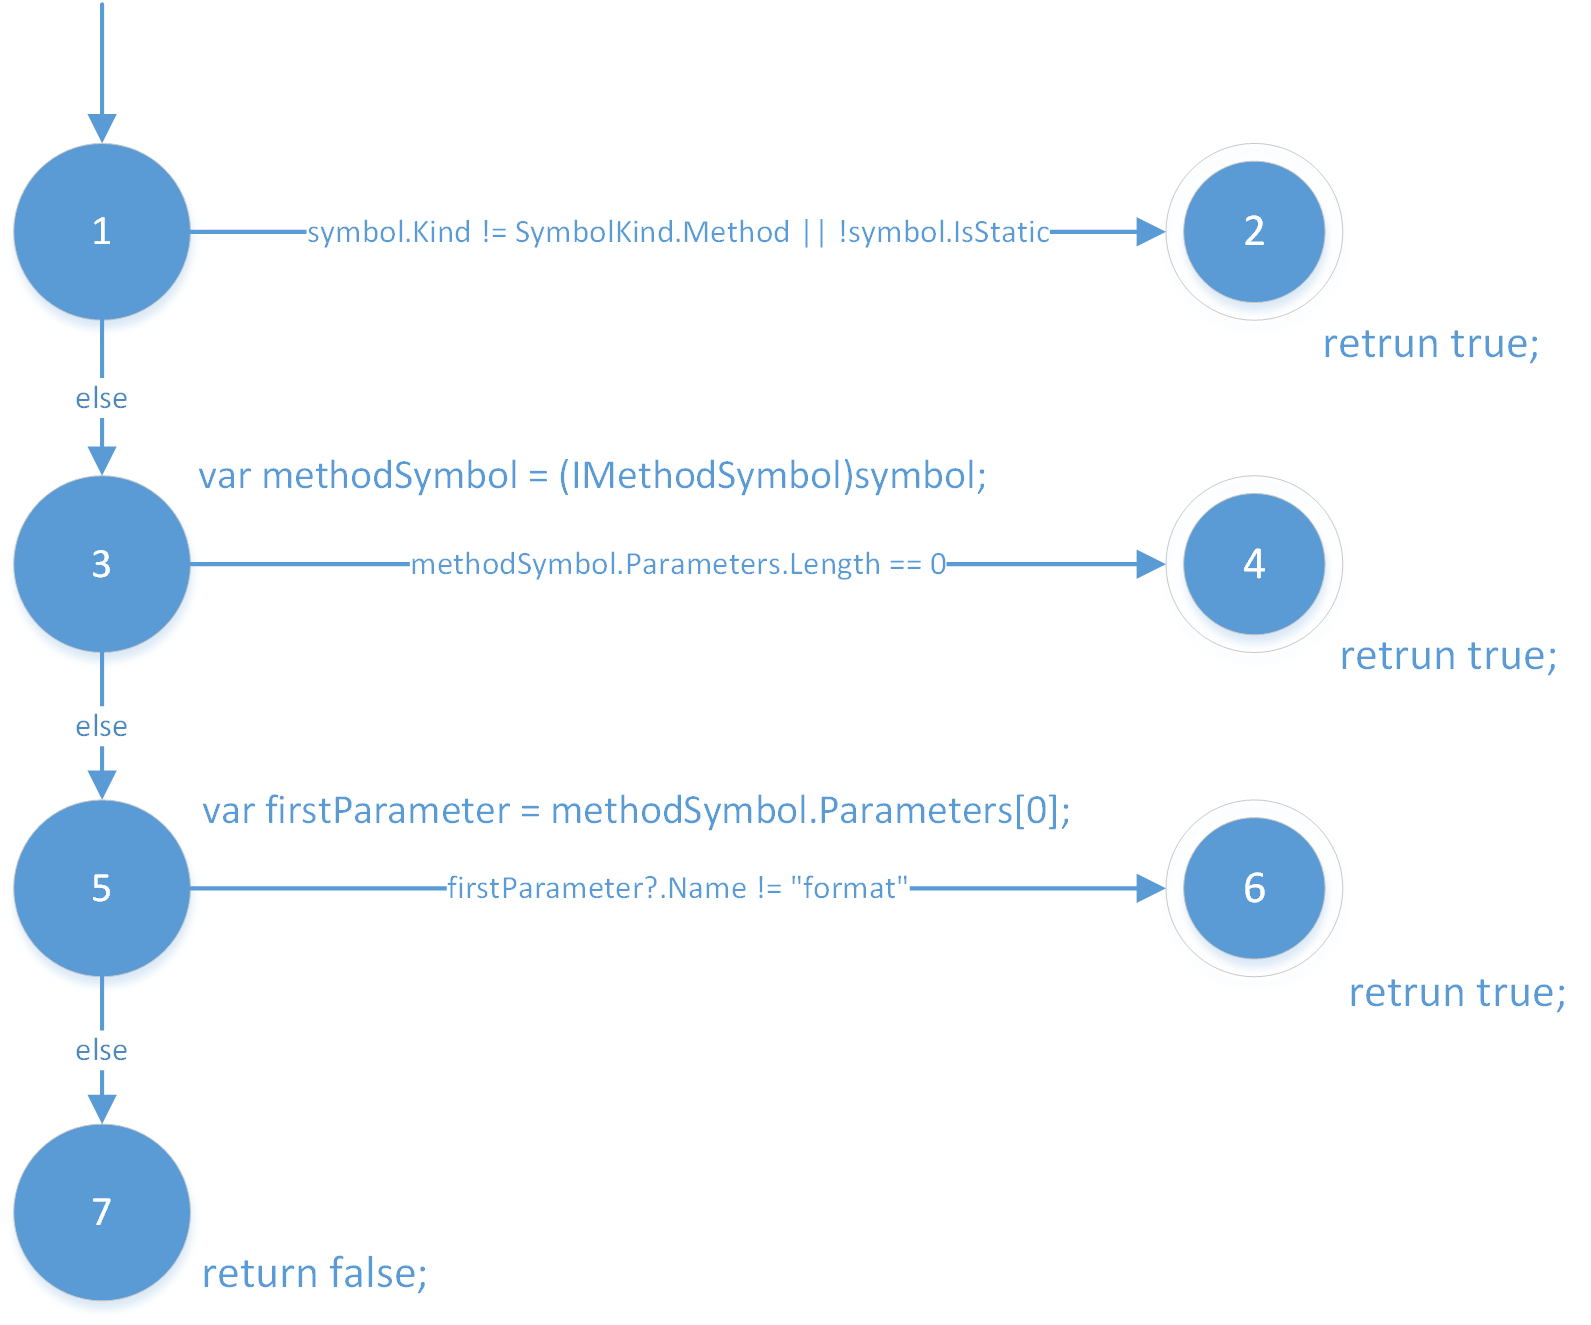
\includegraphics[width=0.8\textwidth]{images/GraphISValidStringFormatMethod.png}
	\caption{Graph für die Methode \texttt{IsValidStringFormatMethod}}
	\label{fig:graph-validstring}
\end{figure}
Auffallend ist, dass alle Coverage Kriterien die selben Testpfade besitzen. Das kommt Zustande, weil die Methode \texttt{IsValidStringFormatMethod} keine Schleifen und Alternativen in den Bedingungen besitzt. Beispielhaft werden die Tests für die Prime Path Coverage an der Implementierung für den Pfad \texttt{[1,3,5,7]} anhand der in Listing \ref{lst:code-ConditionalExpression} abgebildeten Testmethode erläutert. In der Methode werden zwei Codeschnipsel definiert. Der eine wird der Klasse übergeben. Der andere ist das Ergebnis nach der Ausführung. Die Methode \texttt{IsValidStringFormatMethod} gibt bei dem Codeschnipsel \texttt{false} zurück, da der String in einen interpolated String umgewandelt werden kann.

\newpage
\begin{lstlisting}[caption={Mehtode \texttt{IsValidStringFormatMethod}},
label=lst:code-IsValidStringFormatMethod]
private static bool IsValidStringFormatMethod(ISymbol symbol)
{
	if (symbol.Kind != SymbolKind.Method || !symbol.IsStatic)
	{
		return true;
	}
	var methodSymbol = (IMethodSymbol)symbol;
	if (methodSymbol.Parameters.Length == 0)
	{
		return true;
	}
	var firstParameter = methodSymbol.Parameters[0];
	if (firstParameter?.Name != "format")
	{
		return true;
	}
	return false;
}
\end{lstlisting}
\begin{lstlisting}[caption={Mehtode \texttt{ConditionalExpression}},
label=lst:code-ConditionalExpression]
[Test]
public void ConditionalExpression()
{
	const string markupCode = @"
	class C
	{
		void M()
		{
			var s = [|string.Format(""{0}"", 42 == 42 ? true : false)|];
		}
	}";
	const string expected = @"
	class C
	{
		void M()
		{
			var s = $""{(42 == 42 ? true : false)}"";
		}
	}";

	TestCodeRefactoring(markupCode, expected);
}
\end{lstlisting}


\subsection{Fazit}
Das Testen der Methoden des Projekts hat uns gezeigt, dass gutes Testen einiges an Aufwand bedeutet, da es bei komplexen Methoden schwierig sein kann den Kontrollflussgraphen und die zugehörigen Coverage Kriterien aufzustellen. Wir hoffen, dass anhand unsere beispielhaft für einige Methoden geschilderten Vorgehensweise, deutlich geworden wie wir versucht haben Fehler im Projekt zu finden. Die entwickelten und schon vorhandenen Tests haben wir durch bilden von Mutation am ursprünglichen Code selbst getestet. Dabei haben wir einige Zeilen der ursprünglichen Methoden verändert und die Tests auf ihnen laufen lassen. Es hat uns gefreut sehen zu können, dass alle Mutation von den Tests erkannt und gekillt wurden.\\

